\documentclass{article}

% if you need to pass options to natbib, use, e.g.:
%     \PassOptionsToPackage{numbers, compress}{natbib}
% before loading neurips_2018

% ready for submission
% \usepackage{neurips_2018}

% to compile a preprint version, e.g., for submission to arXiv, add add the
% [preprint] option:
%     \usepackage[preprint]{neurips_2018}

% to compile a camera-ready version, add the [final] option, e.g.:
     \usepackage[final]{neurips_2018}

% to avoid loading the natbib package, add option nonatbib:
%     \usepackage[nonatbib]{neurips_2018}

\usepackage[utf8]{inputenc} % allow utf-8 input
\usepackage[T1]{fontenc}    % use 8-bit T1 fonts
\usepackage{hyperref}       % hyperlinks
\usepackage{url}            % simple URL typesetting
\usepackage{booktabs}       % professional-quality tables
\usepackage{amsfonts}       % blackboard math symbols
\usepackage{nicefrac}       % compact symbols for 1/2, etc.
\usepackage{microtype}      % microtypography
\usepackage{amsmath}
\usepackage{amssymb}
\usepackage{graphicx}
\usepackage{subcaption}
\usepackage{booktabs}
\newcommand{\pd}[2]{\frac{\partial #1}{\partial #2}}

\title{Deep Learning\\Assignment 2: Recurrent Neural Networks and Graph Neural Networks}

% The \author macro works with any number of authors. There are two commands
% used to separate the names and addresses of multiple authors: \And and \AND.
%
% Using \And between authors leaves it to LaTeX to determine where to break the
% lines. Using \AND forces a line break at that point. So, if LaTeX puts 3 of 4
% authors names on the first line, and the last on the second line, try using
% \AND instead of \And before the third author name.

\author{%
  Daniel Daza\\
  University of Amsterdam\\
  \texttt{daniel.dazacruz@student.uva.nl} \\
}

\begin{document}
% \nipsfinalcopy is no longer used

\maketitle

\begin{abstract}
-
\end{abstract}

\section{Vanilla RNN versus LSTM}

\subsubsection*{Question 1.1}

The equations for the RNN are the following:

\begin{align}
\mathbf{h}^{(t)} &= \tanh(\mathbf{W}_{hx}\mathbf{x}^{(t)} + \mathbf{W}_{hh}\mathbf{h}^{(t-1)} + \mathbf{b}_h) \label{eq:rnn1}\\
\mathbf{p}^{(t)} &= \mathbf{W}_{ph}\mathbf{h}^{(t)} + \mathbf{b}_p\\
\hat{\mathbf{y}} &= \text{softmax}(\mathbf{p}^{(T)}) \\
\mathcal{L} &= -\sum_{k=1}^K y_{k} \log\hat{y}_k \label{eq:rnn2}
\end{align}

We now calculate the gradient of the loss at time step $T$, with respect to the parameters $\mathbf{W}_{ph}$ and $\mathbf{W}_{hh}$. For brevity we define $\mathbf{p}^{(T)} = \mathbf{p}$.

\begin{equation}
\left(\pd{\mathcal{L}}{\mathbf{W}_{ph}}\right)_{ij} = \sum_u\pd{\mathcal{L}}{\hat{y}_u}\pd{\hat{y}_u}{p_i}\pd{p_i}{(\mathbf{W}_{ph})_{ij}}
\label{eq:dWph}
\end{equation}

\begin{align*}
\pd{\mathcal{L}}{\hat{y}_u} &= \pd{}{\hat{y}_u}\left(-\sum_{k=1}^K y_{k} \log\hat{y}_k\right) \\
&=
\left\lbrace
\begin{matrix}
\pd{}{\hat{y}_u}(-\log \hat{y}_u) & \text{if } u = \arg\max(\hat{y}_u) \\
0 & \text{otherwise}
\end{matrix}
\right.\\
&=
\left\lbrace
\begin{matrix}
-1/\hat{y}_a & \text{if } u = \arg\max(\hat{y}_u) \\
0 & \text{otherwise}
\end{matrix}
\right.
\end{align*}

where we have defined $a = \arg\max(\mathbf{y})$.

\begin{align*}
\pd{\hat{y}_u}{p_i} = \pd{}{p_i}\left(\frac{\exp(p_u)}{\sum_k\exp(p_k)}  \right)
\end{align*}

From assignment 1 we obtain the following result:

\begin{align*}
\pd{\hat{y}_u}{p_i} &=
\left\lbrace
\begin{matrix}
-\hat{y}_u\hat{y}_i & \text{if } i \neq u \\
\hat{y}_i -\hat{y}_u\hat{y}_i & \text{if } i = u
\end{matrix}
\right.
\end{align*}

\begin{align*}
\left(\pd{p_i}{\mathbf{W}_{ph}} \right)_{ij} &= \pd{}{(\mathbf{W}_{ph})_{ij}}(\mathbf{W}_{ph}\mathbf{h}^{(T)} + \mathbf{b}_p)_i \\
&= h^{(T)}_j
\end{align*}

Substituting the previous results in Eq. \ref{eq:dWph}, we obtain

\begin{align*}
\left(\pd{\mathcal{L}}{\mathbf{W}_{ph}}\right)_{ij} &= -\frac{1}{\hat{y}_a} \pd{\hat{y}_a}{p_i}h_j^{(T)} \\
&=
\left\lbrace
\begin{matrix}
-\frac{1}{\hat{y}_a}(-\hat{y}_a\hat{y}_i)h_j^{(T)} & \text{if } i \neq a \\
-\frac{1}{\hat{y}_a}(\hat{y}_a -\hat{y}_a^2)h_j^{(T)} & \text{if } i = a
\end{matrix}
\right.\\
&=
\left\lbrace
\begin{matrix}
\hat{y}_i h_j^{(T)} & \text{if } i \neq a \\
(\hat{y}_a - 1)h_j^{(T)} & \text{if } i = a
\end{matrix}
\right.\\
&= (\hat{y}_i - y_i)h_j^{(T)}
\end{align*}

For the hidden-to-hidden weight matrix, we have

\begin{equation}
\left(\pd{\mathcal{L}}{\mathbf{W}_{hh}}\right)_{ij} = \sum_u\pd{\mathcal{L}}{h_u}\pd{h_u}{(\mathbf{W}_{ph})_{ij}}
\label{eq:dWhh}
\end{equation}

The first term in the sum can be derived from the following results:

\begin{align*}
\pd{\mathcal{L}}{p_i} &= \sum_u\pd{\mathcal{L}}{\hat{y}_u}\pd{\hat{y}_u}{p_i} \\
&= (\hat{y}_i - y_i)
\end{align*}

\begin{align*}
\pd{p_i}{h_u} &= \pd{}{h_u}(\mathbf{W}_{ph}\mathbf{h}^{(T)} + \mathbf{b}_p)_i \\
&= (\mathbf{W}_{ph})_{iu}
\end{align*}

\begin{align*}
\pd{\mathcal{L}}{h_u} &= \sum_i\pd{\mathcal{L}}{p_i}\pd{p_i}{h_u} \\
&= \sum_i(\hat{y}_i - y_i)(\mathbf{W}_{ph})_{iu} \\
&= (\mathbf{W}_{ph}^\top)_{u:}(\hat{\mathbf{y}} - \hat{\mathbf{y}})
\end{align*}

Where the subindex $(\mathbf{W}_{ph}^\top)_{u:}$ denotes a slice with the $u$-th row of $(\mathbf{W}_{ph}^\top)$. The second term in the sum of Eq. \ref{eq:dWhh} is derived next.

\begin{align*}
\pd{h_u}{(\mathbf{W}_{hh})_{ij}} &=
\pd{}{(\mathbf{W}_{hh})_{ij}}\tanh(\mathbf{W}_{hx}\mathbf{x}^{(T)} + \mathbf{W}_{hh}\mathbf{h}^{(T-1)} + \mathbf{b}_h)_u \\
&=
\pd{}{(\mathbf{W}_{hh})_{ij}}\tanh((\mathbf{W}_{hx})_{u:}^\top\mathbf{x}^{(T)} + (\mathbf{W}_{hh})_{u:}^\top\mathbf{h}^{(T-1)} + (\mathbf{b}_h)_u) \\
&=
(1 - (h_u^{(T)})^2) \pd{}{(\mathbf{W}_{hh})_{ij}}\sum_k (\mathbf{W}_{hh})_{uk}h^{(T-1)}_k \\
&=
(1 - (h_u^{(T)})^2) \sum_k\left\lbrace \pd{(\mathbf{W}_{hh})_{uk}}{(\mathbf{W}_{hh})_{ij}}h^{(T-1)}_k + \pd{h_k^{(T-1)}}{(\mathbf{W})_{ij}}(\mathbf{W}_{hh})_{uk}\right\rbrace
\end{align*}

Let $\delta_{ij}$ be 1 if $i=j$ and 0 otherwise. The derivative can then be written as

\begin{equation}
\pd{h_u}{(\mathbf{W}_{hh})_{ij}} =
(1 - (h_u^{(T)})^2) \sum_k\left\lbrace \mathbb{I}[u=i]\mathbb{I}[j=k]  h^{(T-1)}_k + \pd{h_k^{(T-1)}}{(\mathbf{W})_{ij}}(\mathbf{W}_{hh})_{uk}\right\rbrace
\label{eq:explode}
\end{equation}

Where $\mathbb{I}[s]$ is an indicator variable equal to 1 when the statement $s$ is true, and 0 otherwise. Substituting these results in Eq. \ref{eq:dWhh} we can calculate the required gradient:

\begin{equation}
\left(\pd{\mathcal{L}}{\mathbf{W}_{hh}}\right)_{ij} = \sum_u(\mathbf{W}_{ph}^\top)_{u:}(\hat{\mathbf{y}} - \hat{\mathbf{y}})\pd{h_u}{(\mathbf{W}_{ph})_{ij}}
\end{equation}

We observe an important difference in the gradients: while the gradient with respect to $\mathbf{W}_{ph}$ is simpler and depends only on the last time step, the gradient with respect to $\mathbf{W}_{hh}$ depends on the gradients of previous time steps, and at every time step these are multiplied by $\mathbf{W}_{hh}$ (this is shown in Eq. \ref{eq:explode}). Depending on the spectral radius of $\mathbf{W}_{hh}$, the repeated multiplication can lead to vanishing or exploding gradients.

\subsubsection*{Question 1.2}

For this question we implemented the RNN equations as described in equations \ref{eq:rnn1} to \ref{eq:rnn2} using PyTorch, in order to compute the gradients with its automatic differentiation engine. 

We train an RNN in the task of predicting the last digit of a palindrome number. We initialize the weight matrices with a uniform distribution $\mathcal{U}(-1/\sqrt{n_h}, 1/\sqrt{n_h})$, where $n_h$ is the dimension of the hidden state; and biases are initialized with zeros. We use a hidden size of 128, and the RMSProp optimizer with a learning rate of 0.001. We additionally clip the norm of the gradients to a maximum of 10, to avoid exploding gradients, as shown to be of importance in the last sections when doing backpropagation on RNNs.

\subsection*{Question 1.3}

We study the performance of the RNN for sequences of different lengths. We start with sequences of length 5, for which the model achieves an accuracy of 100\% in a small number of iterations. When increasing the length, a smaller learning rate is required, and therefore more iterations are needed to reach the same accuracy. This is shown in Figure \ref{fig:rnn_acc_curves}.

We experiment with increasing sequence lengths, from 4 to 24, and for each length we run 10 experiments in order to evaluate the variance of the results. As shown in Figure \ref{fig:rnn_acc_box}, training on sequences of length 4 yields an accuracy of 100\% almost always. As the length increases, the variance grows as well, and at length 12 we observe the highest variance. This indicates that in this setting, the random initialization of the parameters might produce a very accurate model, or a model with random performance, revealing a high sensitivity on the parameter initialization. For lengths higher than 16 the final performance is consistently lower. These results demonstrate the fact that RNNs are problematic when modeling long sequences.

\begin{figure}[t]
\begin{subfigure}{0.49\textwidth}
\centering
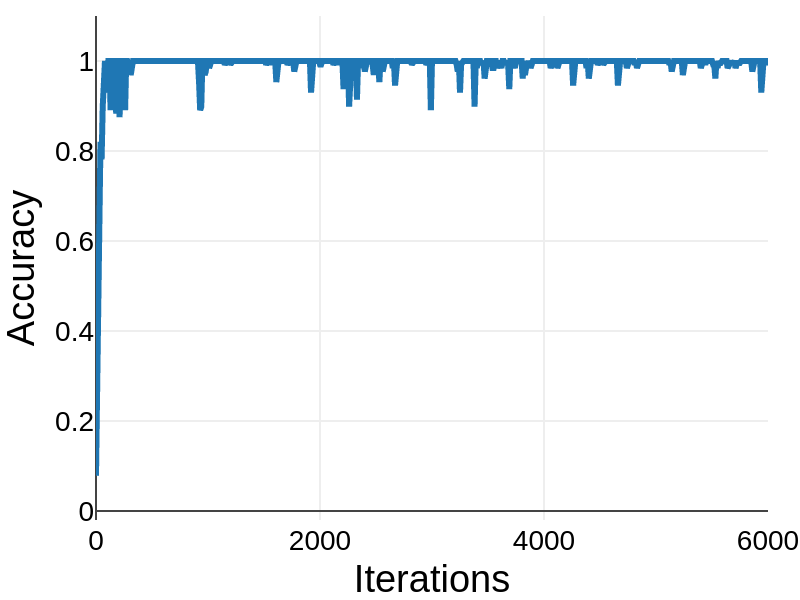
\includegraphics[scale=0.22]{img/rnn-acc-L5}
\caption{}
\end{subfigure}
\begin{subfigure}{0.49\textwidth}
\centering
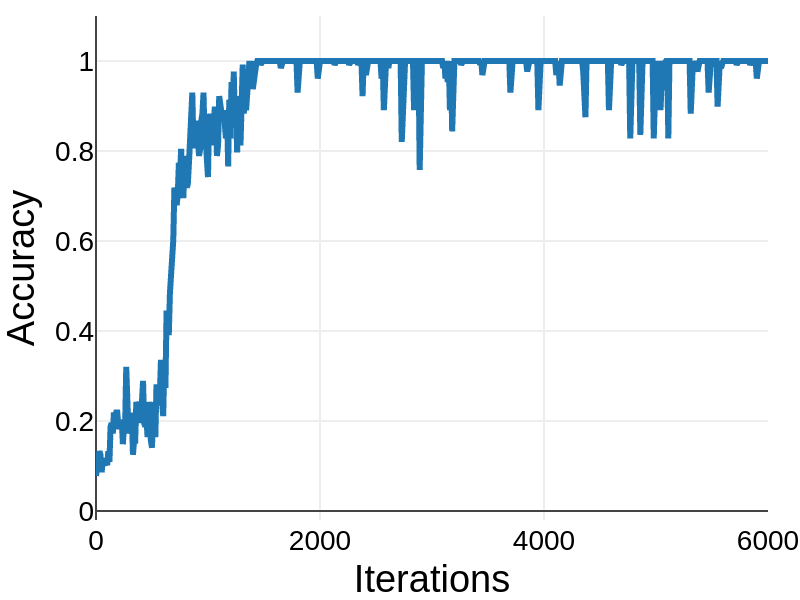
\includegraphics[scale=0.22]{img/rnn-acc-L15}
\caption{}
\end{subfigure}
 \caption{Accuracy curves during training of the RNN, for sequences of (a) length 5, and (b) length 15. While for a length of 5 the model converges quickly to a high accuracy, longer sequences take longer for the model to converge to a good solution.}
\label{fig:rnn_acc_curves}
\end{figure}

\begin{figure}[t]
\centering
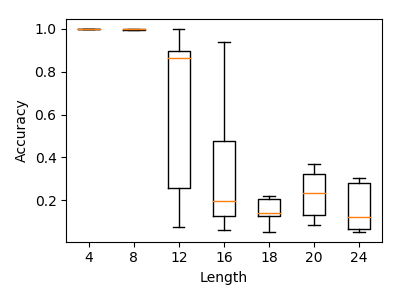
\includegraphics[scale=0.7]{img/rnn-acc-Lbox}
 \caption{Box plots depicting the distribution of the accuracy over 10 runs, for different sequence lengths. As the sequence length increases, obtaining a high accuracy is less likely, and longer sequences tend to random performance.}
\label{fig:rnn_acc_box}
\end{figure}

\subsection*{Question 1.4}

When doing optimization with Stochastic Gradient Descent (SGD), we update the parameters in the direction of the gradient of the loss function. This means that two parameter settings for which the gradient is the same, will be updated equally. This can be a limitation if the curvature of the loss function at the two points is different: if the curvature at a point is very low, the update will produce a small change in the loss, while if the curvature is high, the update can make a change too big in the loss function, which might end up at an even higher point. Therefore, it is sensible to include second order information of the gradient that takes into account the curvature of the loss function when updating the parameters.

A direct way to include second order information is to calculate the Hessian matrix, which contains the second derivatives of the loss with respect to all pairs of parameters in the network. As a consequence, evaluating this matrix has a complexity of $O(W^2)$ where $W$ is the number of parameters \cite{bishop2006pattern}. In deep learning, the number of parameters can be on the order of millions, which motivates finding alternative methods that consider curvature in the parameter updates. Two of these include momentum and adaptive learning rate.

When using momentum, we update the parameters with a moving average of the gradient, instead of the gradient only. In this way, every update takes into account previous values of the gradient, producing updates that are smoother than those of SGD.

In SGD, every parameter is updated with the gradient multiplied by the same learning rate. During training, however, some parameters might be near the values of convergence, whereas other still need to be adjusted. It is thus reasonable to adapt the learning rate to each parameter, so that each one is affected only by its own influence on the loss function. Methods like RMSProp implement this by keeping a moving average of the squared gradients, whose inverse is used to multiply the gradient element-wise, effectively adjusting the gradients on different scales for each parameter.

\subsection*{Question 1.5}

\begin{description}
\item[a)] The LSTM is comprised by four gates:
\begin{itemize}
\item \textbf{Input modulation gate:} This gate prepares the previous hidden state $\mathbf{h}^{(t-1)}$ and the current input $\mathbf{x}^{(t)}$ to be processed for the current time step. It does so by applying a linear transformation to $\mathbf{h}^{(t-1)}$ and $\mathbf{x}^{(t)}$ and passing the result through a nonlinearity. The nonlinearity is required to give the network the ability to model complex a complex function of its input. The $\tanh$ function is a common choice that limits the range to the interval $(-1, 1)$, and constrains the magnitude of inputs of subsequent layers by saturating for large negative or positive inputs.
\item \textbf{Input gate:} This gate determines the amount of the result of the input modulation gate $\mathbf{g}^{(t)}$ that is used to update the current cell state. This amount is determined by a linear transformation of the previous hidden state $\mathbf{h}^{(t-1)}$ and the current input $\mathbf{x}^{(t)}$, passed through a nonlinearity. In this case a sigmoid is used because it maps its inputs to the interval $(0,1)$, so that $\mathbf{g}^{(t)}$ is not used at all, when the input gate is 0, or used in its entirety, when the input gate is 1. The smooth, monotonic increase of the sigmoid function also allows partial use of $\mathbf{g}^{(t)}$.
\item \textbf{Forget gate:} This gate determines how much of the previous cell state is preserved to update the current cell state, as a function of $\mathbf{h}^{(t-1)}$ and $\mathbf{x}^{(t)}$. A sigmoid is used as the nonlinearity for the same reason as the input gate.
\item \textbf{Output gate:} This gate is used to modulate the amount of the updated current cell state used as the new hidden state $\mathbf{h}^{(t)}$, also as a function of $\mathbf{h}^{(t-1)}$ and $\mathbf{x}^{(t)}$, and using the sigmoid nonlinearity for the same reasons.
\end{itemize}

\item[b)] Let $d$ be the dimension of the input, and $n$ the number of units in the LSTM. There are 8 weight matrices in the LSTM with a size of $(n, d)$, and 4 bias vectors of size $n$. Therefore, the number of trainable parameters in the LSTM cell is $8nd + 4b$. If we took into account the linear output layer that calculates $\mathbf{p}^{(t)}$, we would have to add $k(h + 1)$ parameterers, where $k$ is the number of outputs.
\end{description}

\subsection*{Question 1.6}

We implemented the LSTM and trained it in the same way as the RNN. Figure \ref{fig:lstm_acc_curves} shows the accuracy curves for sequences of length 5 and 15. We observe that the network reaches an accuracy of 100\% in both cases. Interestingly, for sequences of length 15, the LSTM requires more iterations than the RNN. We attribute this to the increase in the number of parameters.


\begin{figure}[t]
\begin{subfigure}{0.49\textwidth}
\centering
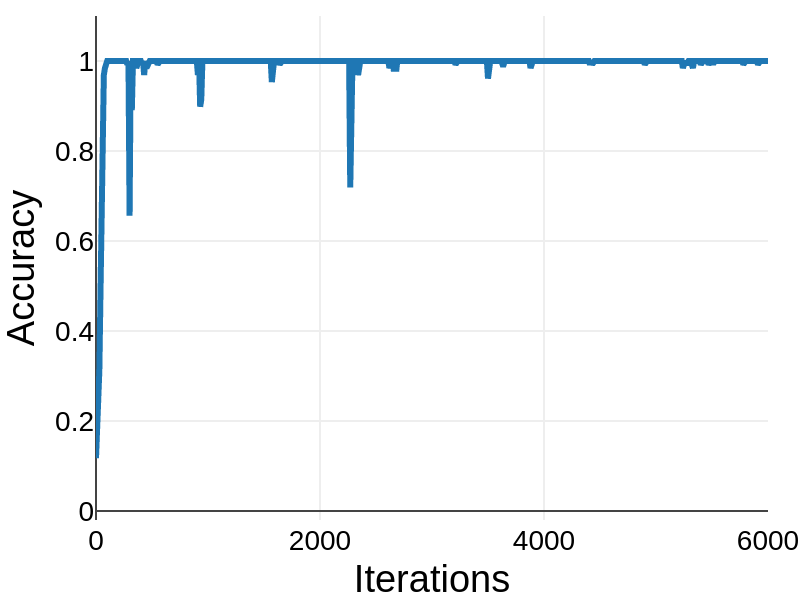
\includegraphics[scale=0.22]{img/lstm-acc-L5}
\caption{}
\end{subfigure}
\begin{subfigure}{0.49\textwidth}
\centering
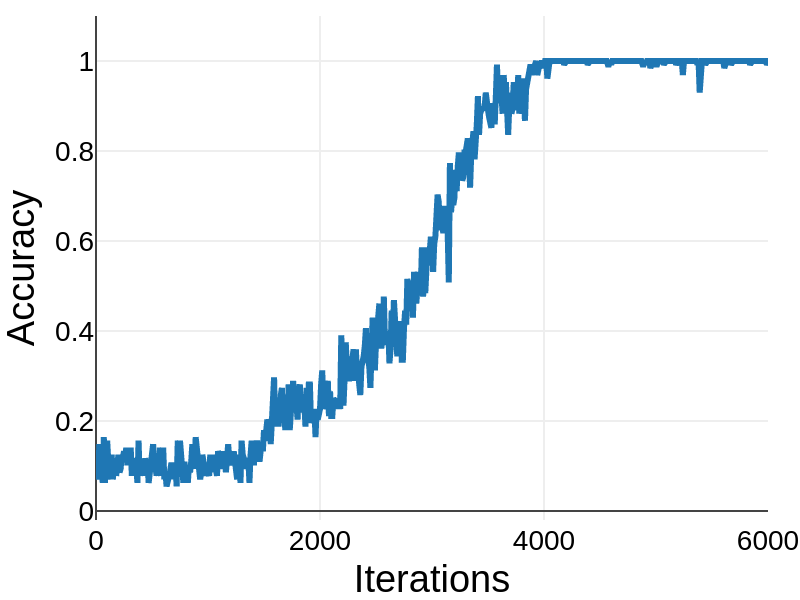
\includegraphics[scale=0.22]{img/lstm-acc-L15}
\caption{}
\end{subfigure}
 \caption{Accuracy curves during training of the LSTM, for sequences of (a) length 5, and (b) length 15. For this setting the LSTM converges more slowly to the solution than the RNN.}
\label{fig:lstm_acc_curves}
\end{figure}




\bibliographystyle{unsrt}
\bibliography{refs}
\end{document}
